In this document, we claim that \glspl{adptSyst} need abstraction to help the reasoning process (\cf \Cref{chapt:intro}).
One way to specify this abstraction is to use the \gls{mde} methodology.
However, as detailed in~\Cref{chapt:intro}, the research community should address different challenges to use state-of-the-art solutions for such systems.
This thesis tackles three of the challenges identified (\cf \Cref{sec:intro:scope}):
\begin{itemize}
	\item How to ease the manipulation of data uncertainty for software engineers?
	\item How to enable reasoning over unfinished actions and their expected effects? (\glspl{longTermAct})
	\item How to model the decisions of an adaptation process to diagnose it?
\end{itemize}

We show in~\Cref{chapt:sota} that it exists no solution to model \gls{longTermAct} or to reason over them.
Besides, we establish that research efforts are still required to handle \gls{duc} at the language level.
To come to this conclusion, we perform a review driven by two research questions (\cf \Cref{sec:sota:methodo}):
\begin{itemize}
	\item \textit{[RQ1]} Do state-of-the-art solutions that model \glspl{adptSyst} allow representing and reasoning over long-term actions?
	\item \textit{[RQ2]} Do state-of-the-art solutions allow modelling uncertainty of data and its manipulation (propagation, reasoning over)?
\end{itemize}

In~\Cref{sec:sota:results:actions}, we answer the first research question.
We first show that the literature provides a few solutions to keep the history of the \gls{structure}, \gls{context}, or \gls{behaviour} of systems~\cite{DBLP:conf/seke/0001FNMKT14, DBLP:conf/models/0001FNMKBT14, 	DBLP:conf/dbpl/MoffittS17, DBLP:conf/icse/TaharaOH17, DBLP:conf/pervasive/HenricksenIR02, DBLP:conf/smartgridsec/0001FKNT14}.
The other solutions, depicted in~\Cref{table:sota:results:actions:rq1.1},  such as goal models~ \cite{DBLP:conf/icse/CailliauL17, DBLP:conf/icse/IftikharW14a, DBLP:conf/icse/MendoncaAR14, DBLP:conf/icse/ChenPYNZ14, DBLP:conf/re/BaresiPS10} or object-based models~\cite{DBLP:conf/pervasive/HenricksenIR02, DBLP:conf/smartgridsec/0001FKNT14, DBLP:conf/icse/TaharaOH17} do not support the time dimension natively.
However, this feature remains important to enable the modelling of \glspl{longTermAct}.
Then, we show that none of the state-of-the-art approaches allows stakeholders to model \glspl{longTermAct}.
Indeed, they do not incorporate a time dimension in their models.
We give an overview of the different solutions in~\Cref{table:sota:results:actions:rq1.2}.
Finally, we show that, using one of the current solutions, one cannot reason over running actions with their expected effects.
Some solution exists to represent action effects at design time.
First, those that employ a state machine~\cite{DBLP:conf/sigsoft/MorenoCGS15, DBLP:conf/kbse/FilieriGLM11,DBLP:conf/wetice/DjoudiBZ14, DBLP:conf/aosd/ZhangGC09, DBLP:conf/icse/GhezziPST13, DBLP:conf/kbse/TajalliGEM10} represent actions as state transitions.
Effects are thus modelled as the target state.
In~\cite{DBLP:conf/smartgridsec/0001FKNT14}, the authors model and use the effects of actions to simulate different sequences of actions.
Lastly, researchers defined the Stitch language~\cite{DBLP:journals/jss/ChengG12} that can abstract action effects.
They are used as conditions for the execution of the next action.
However, none of them models runtime information, useful, for instance, during a diagnosis task.

In~\Cref{sec:sota:results:duc}, we address the second research question.
We first explain that the literature addressed nine kinds of uncertainties, depicted in~\Cref{table:sota:results:duc:rq2.1}.
Among them, the most studied one is the uncertainty relative to data~\cite{DBLP:conf/models/BurguenoBMV18, baudin2017openturns, DBLP:journals/corr/BorgstromGGMG13, DBLP:conf/ecmdafa/BertoaMBBTV18, DBLP:conf/asplos/BornholtMM14, osti_1430202, DBLP:conf/sle/MayerhoferWV16, DBLP:journals/peerj-cs/SalvatierWF16, DBLP:conf/quatic/VallecilloMO16, DBLP:journals/sosym/Zhang00NO19, DBLP:journals/csi/Hall06, DBLP:journals/infsof/Jimenez-RamirezW0V15, DBLP:conf/ecmdafa/ZhangSAYON16, DBLP:journals/tkde/BarbaraGP92, DBLP:conf/vldb/BenjellounSHW06, DBLP:conf/popl/BhatAVG12, DBLP:conf/aistats/ChagantyNR13, DBLP:journals/siamsc/JaroszewiczK12, DBLP:journals/toplas/ParkPT08, DBLP:conf/ijcai/Pfeffer01, DBLP:conf/popl/RamseyP02, DBLP:conf/pldi/SankaranarayananCG13, DBLP:conf/uist/SchwarzMH11, DBLP:conf/icra/Thrun00, DBLP:journals/sac/LunnTBS00, plummer2003jags}.
In this thesis, we also concentrated on this kind of uncertainty.
Then, we detail how researchers model \gls{duc} (\cf \Cref{table:sota:results:duc:rq2.2}).
In our findings, the most used one is the probabilistic programming~\cite{baudin2017openturns, DBLP:conf/asplos/BornholtMM14, DBLP:journals/corr/BorgstromGGMG13, osti_1430202, DBLP:journals/peerj-cs/SalvatierWF16, DBLP:conf/popl/BhatAVG12, DBLP:conf/aistats/ChagantyNR13, DBLP:journals/siamsc/JaroszewiczK12, DBLP:journals/toplas/ParkPT08, DBLP:conf/ijcai/Pfeffer01, DBLP:conf/popl/RamseyP02, DBLP:conf/pldi/SankaranarayananCG13, DBLP:conf/icra/Thrun00, DBLP:journals/sac/LunnTBS00, plummer2003jags}.
Using this programming paradigms, developers can manipulate probability distribution as variables.
They can define complex probability distributions that result from a sequence of operations.
Another approach is to consider a variable as a pair of a standard deviation and a value~\cite{DBLP:conf/models/BurguenoBMV18, DBLP:conf/ecmdafa/BertoaMBBTV18, DBLP:conf/sle/MayerhoferWV16, DBLP:conf/quatic/VallecilloMO16, DBLP:journals/tkde/BarbaraGP92, DBLP:conf/uist/SchwarzMH11}.
Finally, we look for studies that propose a solution to propagate or reason over uncertainty (\cf \Cref{table:sota:results:duc:rq2.3.1}).
The principal approach found to propagate the uncertainty is to map this operation to language operators~\cite{DBLP:conf/models/BurguenoBMV18, baudin2017openturns, DBLP:journals/corr/BorgstromGGMG13, DBLP:conf/ecmdafa/BertoaMBBTV18, osti_1430202, DBLP:conf/sle/MayerhoferWV16, DBLP:journals/peerj-cs/SalvatierWF16, DBLP:conf/quatic/VallecilloMO16, DBLP:conf/popl/BhatAVG12, DBLP:conf/aistats/ChagantyNR13, DBLP:journals/siamsc/JaroszewiczK12, DBLP:journals/toplas/ParkPT08, DBLP:conf/ijcai/Pfeffer01, DBLP:conf/popl/RamseyP02, DBLP:conf/pldi/SankaranarayananCG13, DBLP:conf/icra/Thrun00, DBLP:journals/sac/LunnTBS00, plummer2003jags}.
Concerning reasoning approaches, we find only two ways, as shown in~\Cref{table:sota:results:duc:rq2.3.2}.
The first one consists in giving access to the confidence parameter~\cite{DBLP:conf/models/BurguenoBMV18, DBLP:conf/ecmdafa/BertoaMBBTV18, DBLP:conf/sle/MayerhoferWV16, DBLP:conf/quatic/VallecilloMO16, DBLP:journals/tkde/BarbaraGP92, DBLP:conf/uist/SchwarzMH11}.
The second one is to allow developers to read and manipulate features of the probability distribution~\cite{baudin2017openturns, DBLP:conf/asplos/BornholtMM14, DBLP:journals/corr/BorgstromGGMG13, osti_1430202, DBLP:journals/peerj-cs/SalvatierWF16, DBLP:conf/popl/BhatAVG12, DBLP:conf/aistats/ChagantyNR13, DBLP:journals/siamsc/JaroszewiczK12, DBLP:journals/toplas/ParkPT08, DBLP:conf/ijcai/Pfeffer01, DBLP:conf/popl/RamseyP02, DBLP:conf/pldi/SankaranarayananCG13, DBLP:conf/icra/Thrun00, DBLP:journals/sac/LunnTBS00, plummer2003jags}.\looseness-1

To summarise, our review of the state-of-the-art shows first that research efforts are still necessary to specify a model-based approach for \glspl{longTermAct}.
Besides, it demonstrates that the research community should focus on defining solutions to manipulate uncertain data at a higher level than the manipulation of probability distributions.
We think that both challenges can be addressed by the definition of a modelling framework that includes, despite all traditional elements, temporal and uncertainty as first-class concepts.
We depict this vision in~\Cref{fig:vision:vision}.
Using this framework, designers can define a model adding high-level information about the time and uncertainty.
Then, the framework will automatically generate software artefacts to evaluate, propagate, and reason over uncertainty.
Moreover, artefacts to efficiently store and navigate through complex temporal data structures.
Hartmann~\etal partially implemented this vision~\cite{DBLP:journals/is/HartmannFMRT19}, which led to the \gls{gcm}. 
Using this framework, a modeller will not specify any time-related information in the models.
They will be automatically generated by the framework, with dedicated data structures for temporal data to enable efficient storage and query.

\begin{figure}
	\centering
	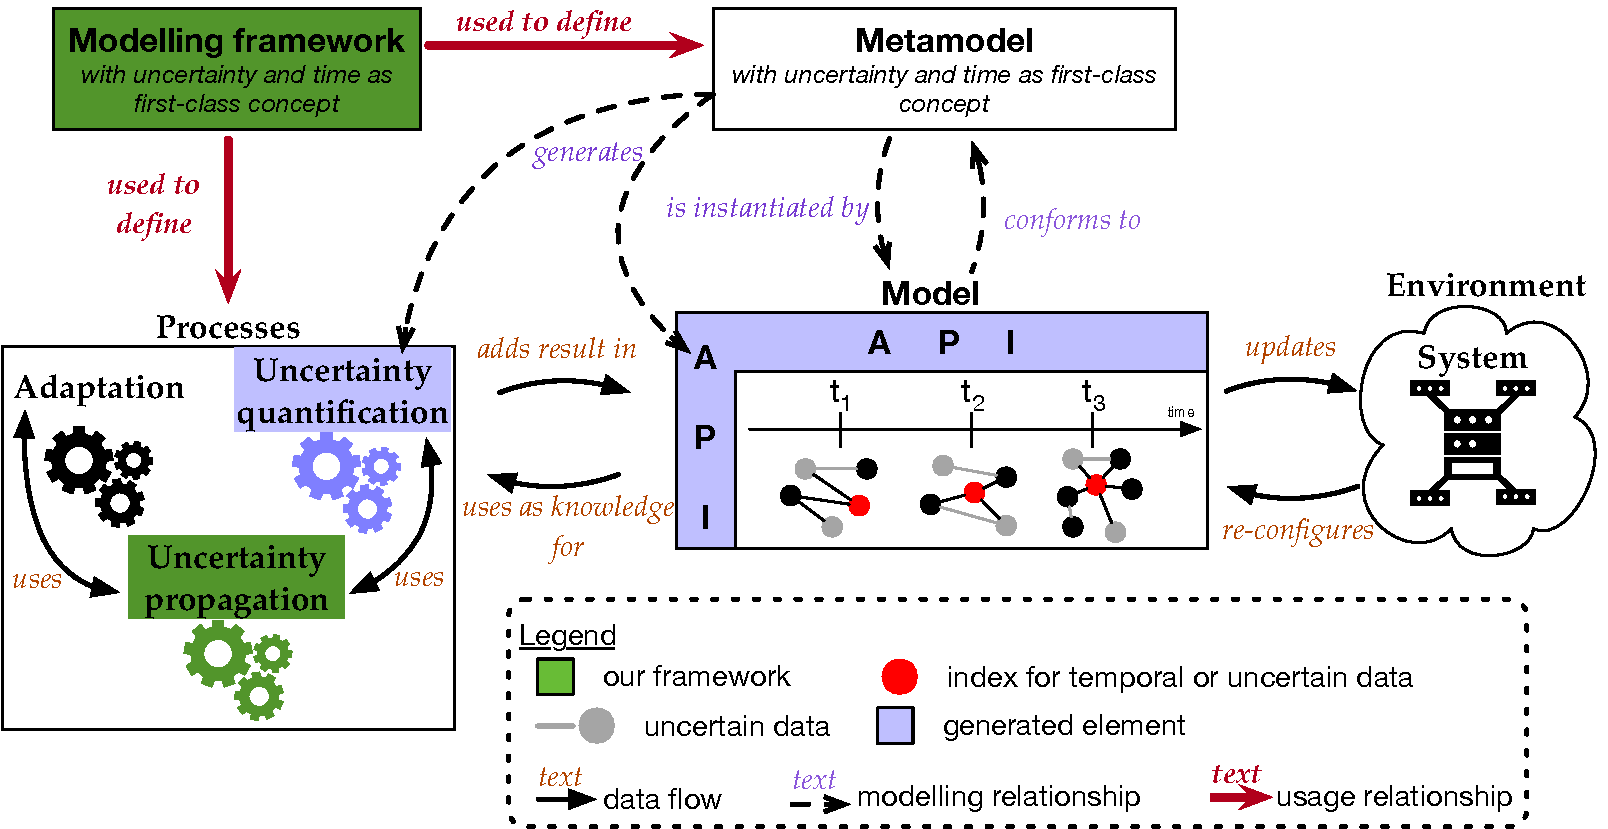
\includegraphics[width=\linewidth]{img/chapt-vision/vision}
	\caption{Overview of our vision}
	\label{fig:vision:vision}
\end{figure}

We present, in this thesis, two contributions towards this vision.
First, we detail our language named \langName{}, which permits designers managing uncertainty at the language level, in~\Cref{chapt:aintea}.
This solution addressed the challenge of the manipulation of uncertain data (cf. Sub-Challenge \#1). 
Second, we describe a temporal knowledge model in~\Cref{chapt:tkm} to structure and store the state and behaviour of a running \gls{adptSyst}, with running \glspl{longTermAct}.
This model addresses the challenge of reasoning over unfinished actions, and understanding of \gls{adptSyst} \gls{behaviour} (cf. Sub-Challenge \#2 and \#3).\looseness-1


